\section{Teilversuch 3: Trägheitsmomente verschiedener Körper}
    \subsection{Kalibrierung des Torsionspendels}
        Fehler bei der Zeitmessung mit Handy $= \SI{0,5}{\second}$

        \textbf{Messreihe}
            \begin{center}
                \begin{tabular}{l rrrr|r}
                    \toprule
                    $n$ & 1 & 2 & 3 & 4 & $\overbar{T_n}/\SI{}{\second}$ \\
                    \midrule
                    $5T_n/\SI{}{\second}$ & \SI{83.12}{} & \SI{82.44}{} & \SI{82.42}{} & \SI{82.24}{} & \SI{16.51}{} \\
                    \bottomrule
                \end{tabular}
            \end{center}
            wobei $\overbar{T_n}$ und seiner zugehöriger Fehler $\Delta \overbar{T_n}$ ist gegeben durch:
            \vspace{-0.5\baselineskip}
            \begin{multicols}{2}
                \begin{equation}
                    \overbar{T_n} = \frac{1}{5n}\sum_{i=1}^n \left(5T_i\right) = \frac{1}{20}\sum_{i=1}^4 \left(5T_i\right) \label{eqn:mittelT}
                \end{equation}
                \begin{equation}
                    \Delta \overbar{T_n} = \frac{\Delta \left(5T\right)}{5\sqrt{n}} = \frac{\Delta \left(5T\right)}{5\sqrt{4}} = \SI{0.05}{\second} \label{eqn:deltaT}
                \end{equation}
            \end{multicols}
            \vspace{-0.5\baselineskip}
            Die Schwingungsdauer $T$ ist dann $\SI{16.51(5)}{\second}$.

        \subsubsection{Rechnung}
            Aus Gleichung (10) und (12) der Anleitung haben wir:
            \begin{align}
                k = \frac{D}{4\pi^2} = \frac{J}{\rule{0pt}{1em}T^2} \overset{(12)}{=} \frac{mR^2}{\rule{0pt}{1em}2T^2} \label{eqn:torsion}
            \end{align}
            Der Fehler $\Delta k$ ist gegeben durch:
            \begin{equation}
                \Delta k = \gausserror{k}{m, R, T}
            \end{equation}
            Die partielle Ableitungen liefern jeweils:
            \begin{align}
                \pdv{k}{T} &= mR^2 (-2) \cdot \frac{1}{2} \cdot T^{-3} = -\frac{mR^2}{T^3} \\
                \pdv{k}{R} &= \frac{m}{2T^2}(2)R = \frac{mR}{T^2} \\
                \pdv{k}{m} &= \frac{R^2}{2T^2}
            \end{align}
            \begin{equation}
                \implies \Delta k = \frac{R}{T^2}\sqrt{\left(\frac{R}{2}\Delta m\right)^2 + \left(m\Delta R\right)^2 + \left(\frac{mR}{T}\Delta T\right)^2}
            \end{equation}
            Mit der folgenden Werten
            \begin{center}
                \begin{tabular}{lrl}
                    \toprule
                    Variable & Wert & Bedeutung \\
                    \midrule
                    $m$ & \SI{3013.80(13)}{\gram} & Masse der Scheibe \\ 
                    $2R$ & \SI{16.9(1)}{\centi\meter} & Durchmesser der Scheibe \\ 
                    $R$ & \SI{8.45(5)}{\centi\meter} & Radius der Scheibe \\ 
                    $T$ & \SI{16.51(5)}{\second} & Schwingungsdauer \\ 
                    \bottomrule
                \end{tabular}
            \end{center}
            lässt sich $k$ und $\Delta k$ bestimmen:
            \begin{align}
                k &= \frac{mR^2}{\rule{0pt}{1em}2T^2} = \frac{\left(\SI{3.01380}{\kilo\gram}\right)\left(\SI{8.45e-2}{\meter}\right)^2}{2\left(\SI{16.51}{\second}\right)^2} = \SI{3.947332445e-5}{\kilo\gram\meter\squared\per\second\squared} \sigfig{6} \\
                \Delta k &= \frac{R}{T^2}\sqrt{\left(\frac{R}{2}\Delta m\right)^2 + \left(m\Delta R\right)^2 + \left(\frac{mR}{T}\Delta T\right)^2} \notag \\
                &= \frac{\SI{8.45e-2}{\meter}}{\left(\SI{16.51}{\second}\right)^2}\left(\left(\left(\frac{\SI{8.45e-2}{\meter}}{2}\right)\left(\SI{1.3e-4}{\kilo\gram}\right)\right)^2 + \left(\left(\SI{3.01380}{\kilo\gram}\right)\left(\SI{5e-4}{\meter}\right)\right)^2 \right. \notag \\
                &~~~~+ \left. \left(\frac{\left(\SI{3.01380}{\kilo\gram}\right)\left(\SI{8.45e-2}{\meter}\right)}{\left(\SI{16.51}{\second}\right)}\left(\SI{0.05}{\second}\right)\right)^2\right)^{\nicefrac{1}{2}} \notag \\
                &= \SI{5.24772e-7}{\kilo\gram\meter\squared\per\second\squared} = \SI{6e-7}{\kilo\gram\meter\squared\per\second\squared} \sigfig{1}
            \end{align}
            Daraus folgt, dass $k = \SI{3.95(6)e-5}{\kilo\gram\meter\squared\per\second\squared}$ ist.

    \subsection{Berechnung der Trägheitsmomente}
        \subsubsection{Messreihe der Schwingungsdauer}
            Fehler bei jeder Messung $= \SI{0.2}{\second}$

            Die Einheiten sind alle Sekunde.
            \vspace{-\baselineskip}
            \begin{multicols}{3}
                \begin{center}
                    \begin{tabular}{lrr|r}
                        \multicolumn{4}{c}{Fläche $(l_1, l_2)$} \\
                        \toprule
                        $n$    & 1 & 2 & $\overbar{T_n}$ \\
                        \midrule
                        $5T_n$ & \SI{36.08}{} & \SI{35.86}{} & \SI{7.194}{} \\
                        \bottomrule
                    \end{tabular}
                \end{center}
                \begin{center}
                    \begin{tabular}{lrr|r}
                        \multicolumn{4}{c}{Fläche $(l_1, l_3)$} \\
                        \toprule
                        $n$    & 1 & 2 & $\overbar{T_n}$ \\
                        \midrule
                        $5T_n$ & \SI{45.69}{} & \SI{45.63}{} & \SI{9.132}{} \\
                        \bottomrule
                    \end{tabular}
                \end{center}
                \begin{center}
                    \begin{tabular}{lrr|r}
                        \multicolumn{4}{c}{Fläche $(l_2, l_3)$} \\
                        \toprule
                        $n$    & 1 & 2 & $\overbar{T_n}$ \\
                        \midrule
                        $5T_n$ & \SI{50.15}{} & \SI{49.95}{} & \SI{10.01}{} \\
                        \bottomrule
                    \end{tabular}
                \end{center}
            \end{multicols}
            \begin{center}
                \begin{tabular}{lrr|r}
                    \multicolumn{4}{c}{Raumdiagonale} \\
                    \toprule
                    $n$    & 1 & 2 & $\overbar{T_n}$ \\
                    \midrule
                    $5T_n$ & \SI{41.01}{} & \SI{41.04}{} & \SI{8.205}{} \\
                    \bottomrule
                \end{tabular}
            \end{center}

            wobei die jeweilige Mittelwerte analog zu Gleichung \eqref{eqn:mittelT} mit $n = 2$ berechnet wurde. 

            Der jeweilige Fehler ist analog zu Gleichung \eqref{eqn:deltaT} wie folgt gegeben:
            \begin{equation}
                \Delta T = \frac{0,2}{5\sqrt{2}} = \SI{0.029}{\second} \label{eqn:Tfehlerfor2}
            \end{equation}

        \subsubsection{Rechnung mittels Schwingungsdauer}
            Aus Gleichung \eqref{eqn:torsion} ist die Trägheitsmoment $J$ gegeben durch:
            \begin{equation}
                J = k T^2
            \end{equation}
            Der Fehler ist laut AMW dann:
            \begin{equation}
                \Delta J = k T^2 \sqrt{\left(\frac{\Delta k}{k}\right)^2 + \left(\frac{2\Delta T}{T}\right)^2}
            \end{equation}
            Mit $k = \SI{3.9473324(524772)e-5}{\kilo\gram\meter\squared\per\second\squared}$ sind die Hauptträgheitsmomente:\\
            \textbf{Fläche} $(l_1, l_2)$ \textbf{mit} $\hat{e}_{1,2} = \hat{e}_z$ 
            \begin{align}
                J &= \left(\SI{3.95473324e-5}{\kilo\gram\meter\squared\per\second\squared}\right)\left(\SI{7.194}{\second}\right)^2 = \SI{2.04429e-3}{\kilo\gram\meter\squared} \sigfig{6} \\
                \Delta J &= \left(\SI{3.95473324e-5}{}\right)\left(\SI{7.194}{}\right)^2 \sqrt{\left(\frac{\SI{5.24772e-7}{}}{\SI{3.95473324e-5}{}}\right)^2 + \left(\frac{2\left(\SI{0.029}{}\right)}{\SI{7.194}{}}\right)^2} \SI{}{\kilo\gram\meter\squared} \notag \\
                &= \SI{3.177e-5}{\kilo\gram\meter\squared} \\
                &\implies J_z = \SI{2.04(4)e-3}{\kilo\gram\meter\squared}
            \end{align}
            \textbf{Fläche} $(l_1, l_3)$ \textbf{mit} $\hat{e}_{1,3} = \hat{e}_y$ 
            \begin{align}
                J &= \left(\SI{3.95473324e-5}{\kilo\gram\meter\squared\per\second\squared}\right)\left(\SI{9.132}{\second}\right)^2 = \SI{3.29182e-3}{\kilo\gram\meter\squared} \sigfig{6} \\
                \Delta J &= \left(\SI{3.95473324e-5}{}\right)\left(\SI{9.132}{}\right)^2 \sqrt{\left(\frac{\SI{5.24772e-7}{}}{\SI{3.95473324e-5}{}}\right)^2 + \left(\frac{2\left(\SI{0.029}{}\right)}{\SI{9.132}{}}\right)^2} \SI{}{\kilo\gram\meter\squared} \notag \\
                &= \SI{4.851e-5}{\kilo\gram\meter\squared} \\
                &\implies J_y = \SI{3.29(5)e-3}{\kilo\gram\meter\squared}
            \end{align}
            \textbf{Fläche} $(l_2, l_3)$ \textbf{mit} $\hat{e}_{2,3} = \hat{e}_x$ 
            \begin{align}
                J &= \left(\SI{3.95473324e-5}{\kilo\gram\meter\squared\per\second\squared}\right)\left(\SI{10.01}{\second}\right)^2 = \SI{3.95523e-3}{\kilo\gram\meter\squared} \sigfig{6} \\
                \Delta J &= \left(\SI{3.95473324e-5}{}\right)\left(\SI{10.01}{}\right)^2 \sqrt{\left(\frac{\SI{5.24772e-7}{}}{\SI{3.95473324e-5}{}}\right)^2 + \left(\frac{2\left(\SI{0.029}{}\right)}{\SI{10.01}{}}\right)^2} \SI{}{\kilo\gram\meter\squared} \notag \\
                &= \SI{5.736e-5}{\kilo\gram\meter\squared} \\
                &\implies J_x = \SI{3.96(6)e-3}{\kilo\gram\meter\squared}
            \end{align}
            \textbf{Raumdiagonale}
            \begin{align}
                J &= \left(\SI{3.95473324e-5}{\kilo\gram\meter\squared\per\second\squared}\right)\left(\SI{8.205}{\second}\right)^2 = \SI{2.65742e-3}{\kilo\gram\meter\squared} \sigfig{6} \\
                \Delta J &= \left(\SI{3.95473324e-5}{}\right)\left(\SI{8.205}{}\right)^2 \sqrt{\left(\frac{\SI{5.24772e-7}{}}{\SI{3.95473324e-5}{}}\right)^2 + \left(\frac{2\left(\SI{0.029}{}\right)}{\SI{8.205}{}}\right)^2} \SI{}{\kilo\gram\meter\squared} \notag \\
                &= \SI{4.00124e-5}{\kilo\gram\meter\squared} \\
                &\implies J_d = \SI{2.66(5)e-3}{\kilo\gram\meter\squared}
            \end{align}
            Genauere $k$ und $T$ wurden hier benutzt, um Rundungsfehler zu vermeiden. 

        \subsubsection{Messreihe der Längen}
            \begin{wrapfigure}{r}{0.3\textwidth}
                \begin{center}
                    \vspace{-3em}
                    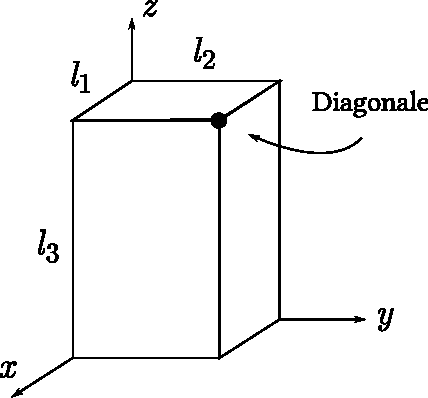
\includegraphics[width=0.25\textwidth]{cube.pdf}
                    \vspace{-3em}
                \end{center}
            \end{wrapfigure}
            Wir definieren die Längen $L_x$, $L_y$, $L_z$ wie im letzten Abschnitt, das heißt:
            \begin{align*}
                L_x &= l_1 = \SI{5.115(5)}{\centi\meter}  \\
                L_y &= l_2 = \SI{7.315(5)}{\centi\meter}  \\
                L_z &= l_3 = \SI{10.250(5)}{\centi\meter}
            \end{align*} 
        \subsubsection{Rechnung mittels Längemessung}
            Aus der Herleitung lassen $J_d$ und den dazu gehörigen Fehler wie folgt berechnen:
            \begin{align}
                J_d &= \frac{1}{L_x^2+L_y^2 + L_x^2}\left(J_xL_x^2 + J_yL_y^2 + J_zL_z^2\right)\\
                \Delta J_d &= \gausserror{J_d}{L_x, L_y, L_z, J_x, J_y, J_z}
            \end{align}
            Sei $r(L_x, L_y, L_z) = L_x^2+L_y^2 + L_x^2$, dann liefern die partielle Ableitungen jeweils:
            \begin{align*}
                \pdv{J_d}{L_x} &= J_x\left(\frac{2L_x}{r}-\frac{L_x^2}{r^2}\pdv{r}{L_x}\right) = \frac{2J_xL_x}{r}\left(1 -\frac{L_x^2}{r}\right) \\
                \pdv{J_d}{L_y} &= \frac{2J_yL_y}{r}\left(1 -\frac{L_y^2}{r}\right) \hspace{2cm} \pdv{J_d}{L_z} = \frac{2J_zL_z}{r}\left(1 -\frac{L_z^2}{r}\right)\\
                \pdv{J_d}{J_x} &= \frac{L_x^2}{r} \hspace{1cm} \pdv{J_d}{J_y} = \frac{L_y^2}{r} \hspace{1cm} \pdv{J_d}{J_z} = \frac{L_z^2}{r}
            \end{align*}
            Da $(1-L_x^2/r) = (1/r)(r - L_x^2)$ und $\Delta L_x = \Delta L_y = \Delta L_z =\Delta L$. können wir den Fehler so vereinfachen\footnote{Es ist so geschrieben, sodass die Gleichung in einer Zeile geschrieben werden kann. Damit ist die Rechnung auch einfacher. Es gibt keine physikalische Bedeutung.}:
            \begin{align}
                \Delta J_d &= \sqrt{\frac{4\Delta L^2}{r^4} \left(\begin{bmatrix}J_x\left(r-L_x^2\right)\\J_y\left(r-L_y^2\right)\\J_z\left(r-L_z^2\right)\end{bmatrix}\cdot\begin{bmatrix}L_x\\L_y\\L_z\end{bmatrix}\right)^2 + \frac{1}{r^2}\left(\begin{bmatrix}L_x^2\\L_y^2\\L_z^2\end{bmatrix}\cdot\begin{bmatrix}\Delta J_x\\\Delta J_y\\\Delta J_z\end{bmatrix}\right)^2} \notag \\
                &= \frac{1}{r}\sqrt{\frac{4\Delta L^2}{r^2} \left(\begin{bmatrix}J_x\left(r-L_x^2\right)\\J_y\left(r-L_y^2\right)\\J_z\left(r-L_z^2\right)\end{bmatrix}\cdot\begin{bmatrix}L_x \\L_y \\L_z\end{bmatrix}\right)^2 + \left(\begin{bmatrix}L_x^2\\L_y^2\\L_z^2\end{bmatrix}\cdot\begin{bmatrix}\Delta J_x\\\Delta J_y\\\Delta J_z\end{bmatrix}\right)^2}
            \end{align}

            Mithilfe eines \texttt{Python} Skript (Siehe Appendix \ref{appdx:pythonJd}) wurden $J_d$ und $\Delta J_d$ berechnet und wir erhalten $J_d = \SI{2.68(6)e-3}{\kilo\gram\meter\squared}$.

            Tabuliert haben wir:
            \begin{center}
                \begin{tabular}{lr}
                    \toprule
                    $J_d$ (Schwingungsdauer) & \SI{2.66(5)e-3}{\kilo\gram\meter\squared} \\
                    $J_d$ (Rechnung) & \SI{2.68(6)e-3}{\kilo\gram\meter\squared} \\
                    \bottomrule
                \end{tabular}
            \end{center}
            Die Werte stimmen miteinander überein.

        \subsubsection{Rechnung der Hauptträgheitsmoment mittels Längemessung}
            Aus Seite 10 der Anleitung sind die Hauptträgheitsmomente gegeben durch:
            \begin{equation}
                J_x = \frac{1}{12}m\left(L_y^2 + L_z^2\right),\hspace{0.5cm}
                J_y = \frac{1}{12}m\left(L_z^2 + L_x^2\right),\hspace{0.5cm}
                J_z = \frac{1}{12}m\left(L_x^2 + L_y^2\right)
            \end{equation}
            Der Fehler für $J_x$ ist dann:
            \begin{align}
                \Delta J_x = \gausserror{J_x}{m, L_y, L_z}
            \end{align}
            mit $J_y$ und $J_z$ analog. 

            Die partielle Ableitungen liefern jeweils:
            \begin{align}
                \pdv{J_x}{m} = &\frac{1}{12}\left(L_y^2 + L_z^2\right),\hspace{0.5cm}
                \pdv{J_x}{L_y} = \frac{1}{6}mL_y,\hspace{0.5cm}
                \pdv{J_x}{L_z} = \frac{1}{6}mL_z \\
                \Delta J_x &= \sqrt{\frac{1}{144}\left(\left(L_y^2 + L_z^2\right) \Delta m\right)^2 + \frac{m^2\Delta L^2}{36}\left(L_y^2 + L_z^2\right)} \notag \\
                &= \frac{\sqrt{L_y^2 + L_z^2}}{12}\sqrt{\left(L_y^2 + L_z^2\right)\left(\Delta m\right)^2 + \left(4m^2\Delta L^2\right)}
            \end{align}
            mit $J_y$ und $J_z$ analog. 

            Mit $m = \SI{3.01120(13)}{\kilo\gram}$, haben wir:

            \textbf{Fläche} $(l_2, l_3)$ \textbf{mit} $\hat{e}_{2,3} = \hat{e}_x$ 
            \begin{align}
                J_x &= \frac{1}{12}\left(\SI{3.01120}{\kilo\gram}\right)\left(\left(\SI{7.315e-2}{\meter}\right)^2 + \left(\SI{10.250e-2}{\meter}\right)^2\right) \notag \\
                &= \SI{3.97909e-3}{\kilo\gram\meter\squared} \sigfig{6} \\
                \Delta J_x &= \frac{\sqrt{\left(\SI{7.315e-2}{}\right)^2 + \left(\SI{10.250e-2}{}\right)^2}}{12} \notag \\
                &~~~~\times\sqrt{\left(\left(\SI{7.315e-2}{}\right)^2 + \left(\SI{10.250e-2}{}\right)^2\right)\left(\SI{1.3e-4}{}\right)^2 + \left(4\left(\SI{3.01120}{}\right)^2\left(\SI{5e-5}{}\right)^2\right)} ~\SI{}{\kilo\gram\meter\squared} \notag \\
                &= \SI{3.17e-6}{\kilo\gram\meter\squared} \sigfig{3} \\
                &\implies J_x = \SI{3.979(4)e-3}{\kilo\gram\meter\squared}
            \end{align}
            \textbf{Fläche} $(l_1, l_3)$ \textbf{mit} $\hat{e}_{1,3} = \hat{e}_y$ 
            \begin{align}
                J_y &= \frac{1}{12}\left(\SI{3.01120}{\kilo\gram}\right)\left(\left(\SI{5.115e-2}{\meter}\right)^2 + \left(\SI{10.250e-2}{\meter}\right)^2\right) \notag \\
                &= \SI{3.29289e-3}{\kilo\gram\meter\squared} \sigfig{6} \\
                \Delta J_y &= \frac{\sqrt{\left(\SI{5.115e-2}{}\right)^2 + \left(\SI{10.250e-2}{}\right)^2}}{12} \notag \\
                &~~~~\times\sqrt{\left(\left(\SI{5.115e-2}{}\right)^2 + \left(\SI{10.250e-2}{}\right)^2\right)\left(\SI{1.3e-4}{}\right)^2 + \left(4\left(\SI{3.01120}{}\right)^2\left(\SI{5e-5}{}\right)^2\right)} ~\SI{}{\kilo\gram\meter\squared} \notag \\
                &= \SI{2.88e-6}{\kilo\gram\meter\squared} \sigfig{3} \\
                &\implies J_y = \SI{3.293(29)e-3}{\kilo\gram\meter\squared}
            \end{align}
            \textbf{Fläche} $(l_1, l_2)$ \textbf{mit} $\hat{e}_{1,2} = \hat{e}_z$ 
            \begin{align}
                J_z &= \frac{1}{12}\left(\SI{3.01120}{\kilo\gram}\right)\left(\left(\SI{5.115e-2}{\meter}\right)^2 + \left(\SI{7.315e-2}{\meter}\right)^2\right) \notag \\
                &= \SI{1.99925e-3}{\kilo\gram\meter\squared} \sigfig{6} \\
                \Delta J_z &= \frac{\sqrt{\left(\SI{5.115e-2}{}\right)^2 + \left(\SI{10.250e-2}{}\right)^2}}{12} \notag \\
                &~~~~\times\sqrt{\left(\left(\SI{5.115e-2}{}\right)^2 + \left(\SI{10.250e-2}{}\right)^2\right)\left(\SI{1.3e-4}{}\right)^2 + \left(4\left(\SI{3.01120}{}\right)^2\left(\SI{5e-5}{}\right)^2\right)} ~\SI{}{\kilo\gram\meter\squared} \notag \\
                &= \SI{2.24e-6}{\kilo\gram\meter\squared} \sigfig{3} \\
                &\implies J_z = \SI{1.999(23)e-3}{\kilo\gram\meter\squared}
            \end{align}
            \textbf{Vergleichung}
            \begin{center}
                \begin{tabular}{l r r}
                    \toprule
                    & Schwingung & Längemessung \\
                    \midrule
                    $J_x$ & \SI{3.96(6)e-3}{\kilo\gram\meter\squared} & \SI{3.979(4)e-3}{\kilo\gram\meter\squared} \\
                    $J_y$ & \SI{3.29(5)e-3}{\kilo\gram\meter\squared} & \SI{3.293(29)e-3}{\kilo\gram\meter\squared} \\
                    $J_z$ & \SI{2.04(4)e-3}{\kilo\gram\meter\squared} & \SI{1.999(23)e-3}{\kilo\gram\meter\squared} \\
                    \bottomrule
                \end{tabular}
            \end{center}
            Die Fehlerintervalle der Trägheitsmomente jeder Achse überschneidet sich. Die Werte stimmen miteinander überein.